\documentclass[10pt,twocolumn,letterpaper]{article}

\usepackage{ae}%
\usepackage{amsmath}
\usepackage{cvpr}
\usepackage{times}
\usepackage{epsfig}
\usepackage{graphicx}
\usepackage{amsmath}
\usepackage{amssymb}
\usepackage[utf8]{inputenc}


\usepackage[breaklinks=true,bookmarks=false]{hyperref}

\cvprfinalcopy % *** Uncomment this line for the final submission

\def\cvprPaperID{****} % *** Enter the CVPR Paper ID here
\def\httilde{\mbox{\tt\raisebox{-.5ex}{\symbol{126}}}}

\setcounter{page}{1}
\begin{document}

%%%%%%%%% TITLE
\title{\ MÉTODOS DE SEGMENTACIÓN}

\author{K. Guarin \\
University of Los Andes\\
{\tt\small gk.guarin10@uniandes.edu.co}
% For a paper whose authors are all at the same institution,
% omit the following lines up until the closing ``}''.
% Additional authors and addresses can be added with ``\and'',
% just like the second author.
% To save space, use either the email address or home page, not both
}
\maketitle
%\thispagestyle{empty}
%%%% %%%%% ABSTRACT
\begin{abstract}
 La segmentación de imágenes juega un papel muy importante en visión artificial o visión por computador, donde los objetivos principales son poder crear súper píxeles para extraer objetos hasta llegar a satisfacer las necesidades o metas del observador.
 Hasta el día de hoy se han estudiado diferentes métodos en los que se incluyen el agrupamiento de las imágenes digitales, ya sea mediante la utilización de clúster que asocian semejanzas de los píxeles o mediante la jerarquía estimando con el nivel de gris,
 tono o luminancia interpretado como la altitud del relieve en una imagen. En este trabajo se realizó la implementación de 3 técnicas de segmentación de imágenes digitales, utilizando diferentes espacios de color, y luego se evaluaron los métodos propuestos
 y se compararon con métodos avanzados. Se encontró que para la función planteada la técnica de gmm aplicada a un espacio lab proporciona un mejor IDS (optimal image scale) y ODS(optimal dataset scale) que las demás técnicas propuestas.
\\
\\
   {\bf Palabras clave:} segmentación, k-means, gmm, watershed, hsv, lab, precisión, cobertura.
   
   \end{abstract}

%%%%%%%%% BODY TEXT
\section{Introducción}

La visión artificial como ciencia de la computación engloba diferentes técnicas para el procesamiento digital de imágenes, buscando día a día que los 
computadores puedan interpretar las imágenes como las perciben los seres humanos. Con el enorme momento del big data y la diversidad de aplicaciones 
en las que es necesario el uso de imágenes, es posible evidenciar como el estudio de diferentes técnicas de segmentación y en general de procesamiento
de imágenes se ha acrecentado. Los algoritmos de segmentación generalmente se basan en el análisis y procesamiento de una de dos propiedades básicas de
los valores de intensidad: la discontinuidad(cambios abruptos en la intensidad) y similitud (regiones similares según un conjunto de criterios predefinidos).
La segmentación de imágenes significa subdividir en regiones u objetos para permitir de una u otra forma “mejorar” una imagen para posteriormente ser analizada a 
profundidad y poder comprender los objetos en el campo de visión. 
\\
\\
En la actualidad se han desarrollado variados métodos de segmentación para diferentes aplicaciones como la reconstrucción 3D de modelos anatómicos a partir de técnicas de clustering\cite{RODRIGUEZ1997},
la implementación de watershed y fuzzy means para la segmentación y detección de patrones irregulares en imágenes de resonancia magnética\cite{1633722} y la aplicación de la segementación de imágenes de cartilago articular en osteoartrítis\cite{5071225}.
La variabilidad de aplicaciones enel campo de la biomédicina nos muestrá la gran utilidad de la visión artificial y la importancia de entender y conocer las últimas metodologías para el procesamiento de las imágenes.
\newline

El presente trabajo muestra 3 métodos de segementación de imágenes implementados en la base de datos de berkeley.


\subsection{Métodos}
\textbf{K-means}
\\
Es una de las técnicas de agrupamiento más simples usadas en la segmentación de datos e imágenes, cuyo objetivo principal es dividir elementos en grupos o clústers, donde cada
elemento del grupo es similar a otro elemento del mismo grupo. El centroide es el valor o vector característico de cada grupo y representa el “centro” del grupo, dado que los
grupos generalmente tienen forma circular.
\begin{equation}\label{eq:1}
\sum_{i=0}^k \sum_{x_j\in S_i}||x_{i}-u_{i}||^2 
\end{equation}
\newline
\\
$Algoritmo:$
\begin{enumerate}
\item Selecciona el número de grupos.
\item Asigna elementos a cada clúster.
\item Computa nuevos centroides.
\item Itera hasta obtener una estabilidad en las asignaciones.
\end{enumerate}

\textbf{Gmm}
\\
Técnica basada en la representación de cada grupo como una distribución gaussiana; los clúster son formados por la representación de la función de densidad de probabilidad.
La distancia de un punto a otro está dada por el cálculo de la distancia de Mahalanobis, lo cual permite que la distancia se adapte a la distribución de los datos. 
\newline
\\
\begin{equation}
 \sum_{k} \pi_{k}\frac{1}{\sum_k} e^{-d(x,\mu_k;\sum_k)}
\end{equation}
$Algoritmo:$
\begin{enumerate}
\item Seleccionar el número de grupos.
\item Asigna una densidad de probabilidad por grupo.
\item Calcula la distancia euclidiana.
\item Asigna responsabilidades a cada punto.
\item Itera hasta converger a un mínimo local.
\end {enumerate}

\textbf{Watershed}
\newline
Es una técnica de segmentación inspirada en las cuencas hidrográficas, donde la cuenca representa
el conjunto de puntos en los que todas las gotas de lluvia convergen a la misma ubicación. 
las líneas del watershed separan dos cuencas.
En imágenes el tono se interpreta como la altitud de relieve en una imagen y para calcular las cuencas 
se toman los mínimos regionales y se realiza la inundación hasta el nivel deseado.
\newline
\\
$Algoritmo$

\begin{enumerate}
 \item Se hace un agujero para cada mínimo regional de la superficie topográfica.
 \item Se sumerge en agua poco a poco la superficie.
 \item Se van formando lagos y cuando los lagos se encuentran se ubica una línea para evitar que los dos lagos se unan.
 \item El conjunto de presas de agua son las cuencas. 
 \end{enumerate}

\subsection{Espacios de color}

Las imágenes pueden ser representadas en tres espacios de color:

\begin{itemize}
 \item  RGB: Modelo basado en la síntesis de la mezcla por adición de los 3 colores primarios cian, magenta, amarillo 
y negro, además de sus tres componentes espectrales primarias (rojo verde azul).
\end{itemize}

\begin{itemize}
 \item HSV: Se define como el color en términos de sus componentes, o transformación lineal del espacio rgb. Este espacio tiene en cuenta el tinte, saturación y valor.
\end{itemize}

\begin{itemize}
 \item LAB: Modelo cromático para representar todos los colores que puede percibir el ojo humano. L es la luminosidad, a es variación entre rojizo y verdoso, y b la variación entre amarillo y azul.

\end{itemize}


%------------------------------------------------------------------------
\section{Resultados}

De los resultados obtenidos se muestran inicialmente las imágenes para el análisis de la clusterización mediante vecindades
para diferentes espacios de color. En segunda medida se presentan resultados de los 3 métodos de segmentación implementados
(k-means, gmm y watershed) para los tres espacios de color (rgb, hsv y lab). Por último se muestra los resultados a manera comparativa de la evaluación.

\begin{itemize}
 \item Espacios de representación rgb, hsv, lab, rgb+xy, hsv+xy,  lab+xy
 \end{itemize} 

\begin{figure}[h]
\begin{center}
   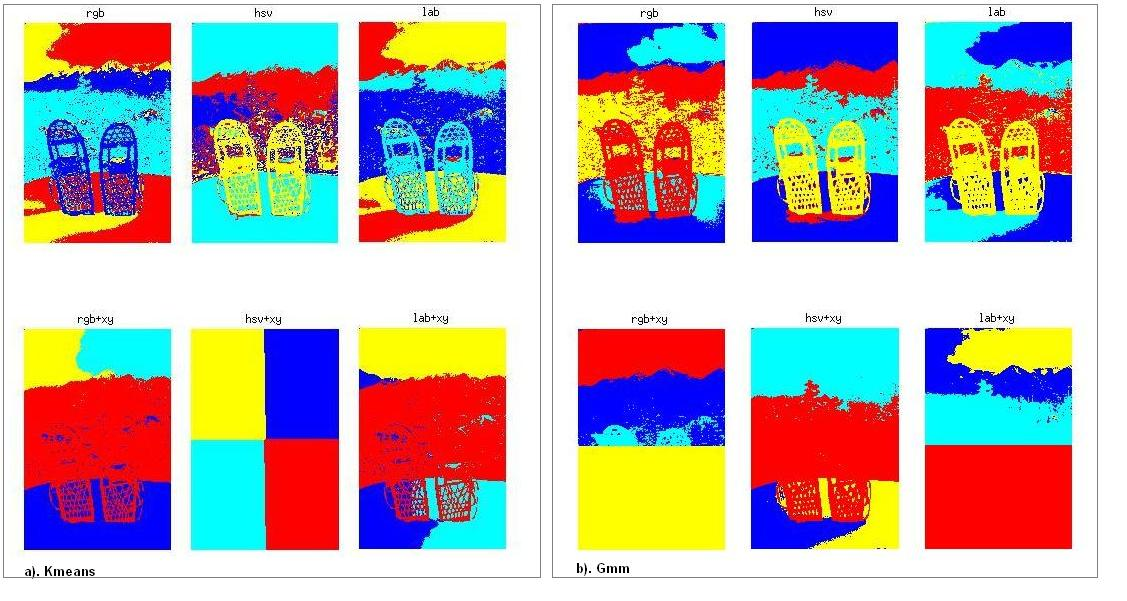
\includegraphics[scale=0.3]{pru.JPG}
\end{center}
   \caption{Espacios de color para k-means y gmm con mismo número de k }
\label{fig:long}
\label{fig:onecol}
\end{figure}
%%%%%%%%%%%%%%%%%%%%%%%%%%5
\begin{itemize}
 \item Métodos de segmentación
\end{itemize}
En las figuras 2, 3, 4, 5 y 6 se presentan resultados de la segmentación para cada método en los diferentes espacios de color.
\begin{figure}[h]
\begin{center}
   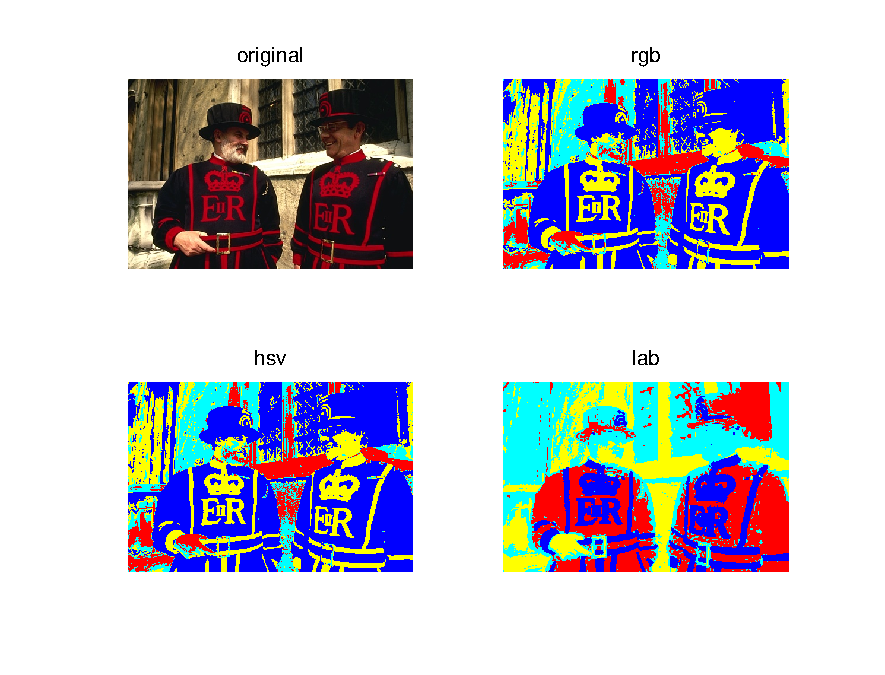
\includegraphics[scale=0.6]{kmeans1.eps}
\end{center}
   \caption{Método kmeans y espacios de color para K=4 }
\label{fig:long}
\label{fig:onecol}
\end{figure}

\begin{figure}[h]
\begin{center}
   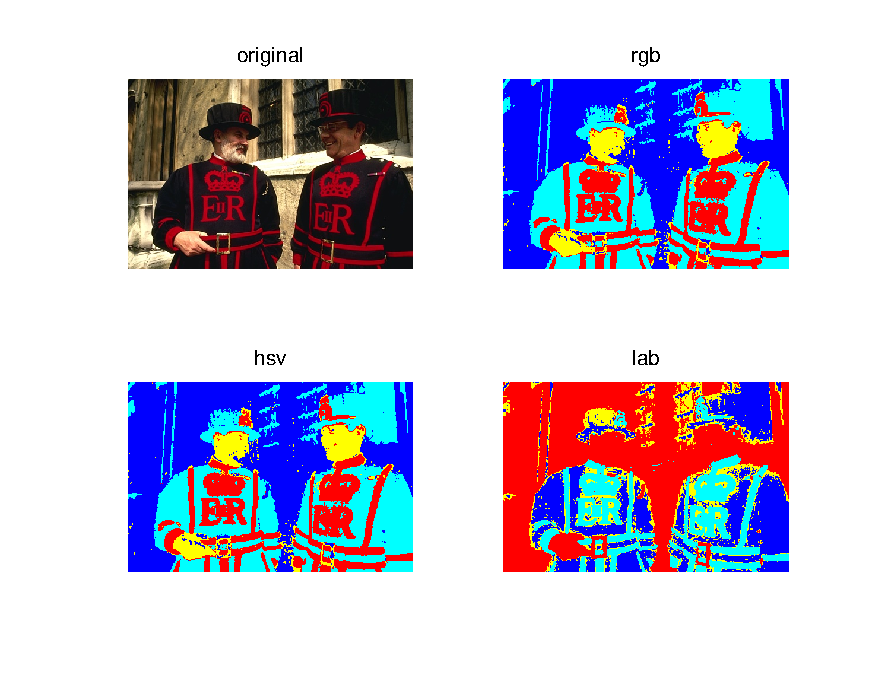
\includegraphics[scale=0.6]{gmm1.eps}
\end{center}   \caption{Método Gmm y espacios de color para K=4 }
\label{fig:long}
\label{fig:onecol}
\end{figure}

\begin{figure}[h]
\begin{center}
   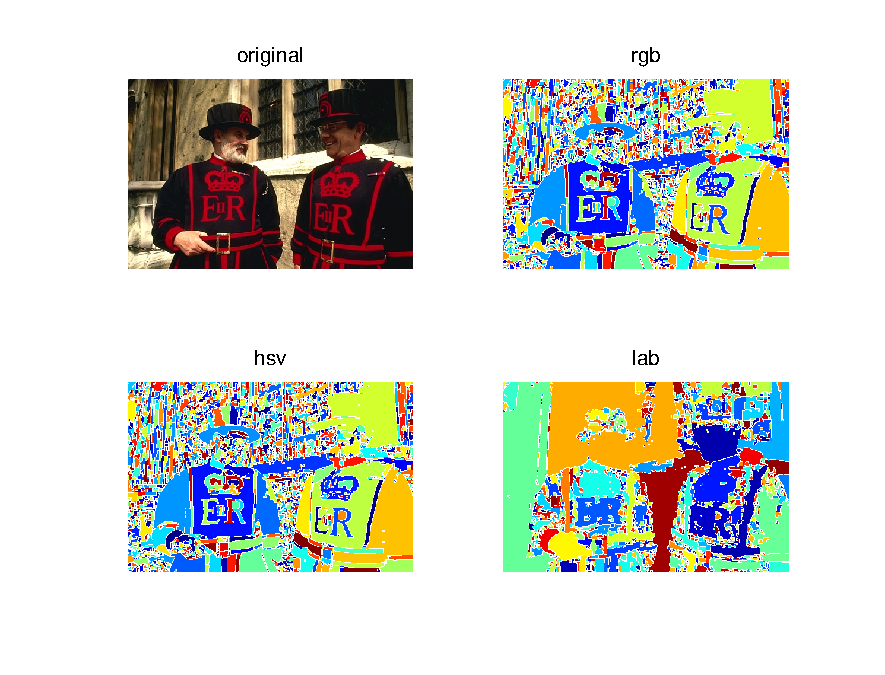
\includegraphics[scale=0.6]{watershed1.eps}
\end{center}
   \caption{Método watershed y espacios de color con h=20. }
\label{fig:long}
\label{fig:onecol}
\end{figure}

\begin{figure}[h]
\begin{center}
 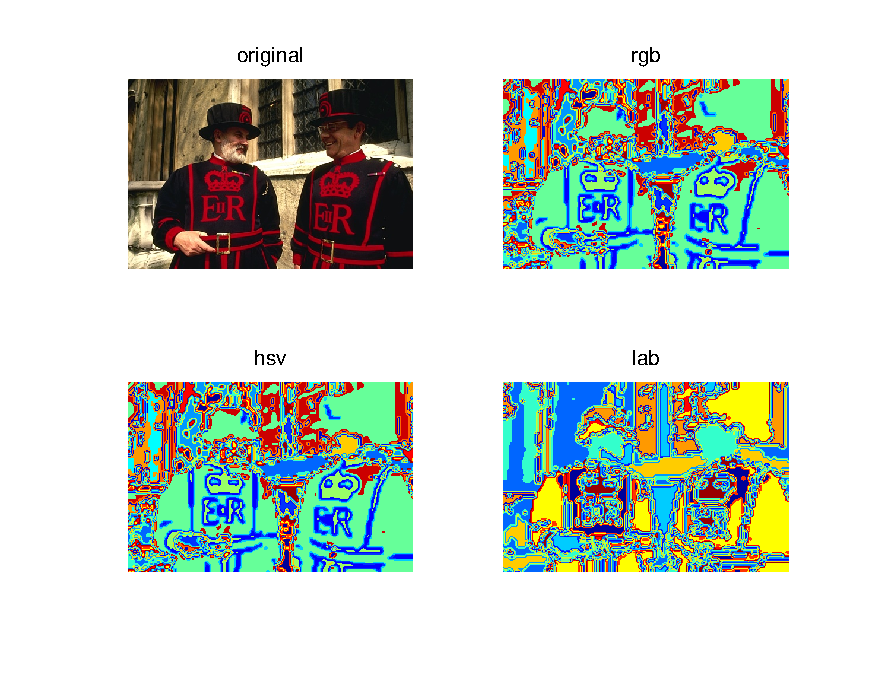
\includegraphics[scale=0.6]{hierarchical1.eps}
\end{center}
   \caption{Método jerarquico y espacios de color con h=20. }
\label{fig:long}
\label{fig:onecol}
\end{figure}

\begin{figure}[h]
\begin{center}
 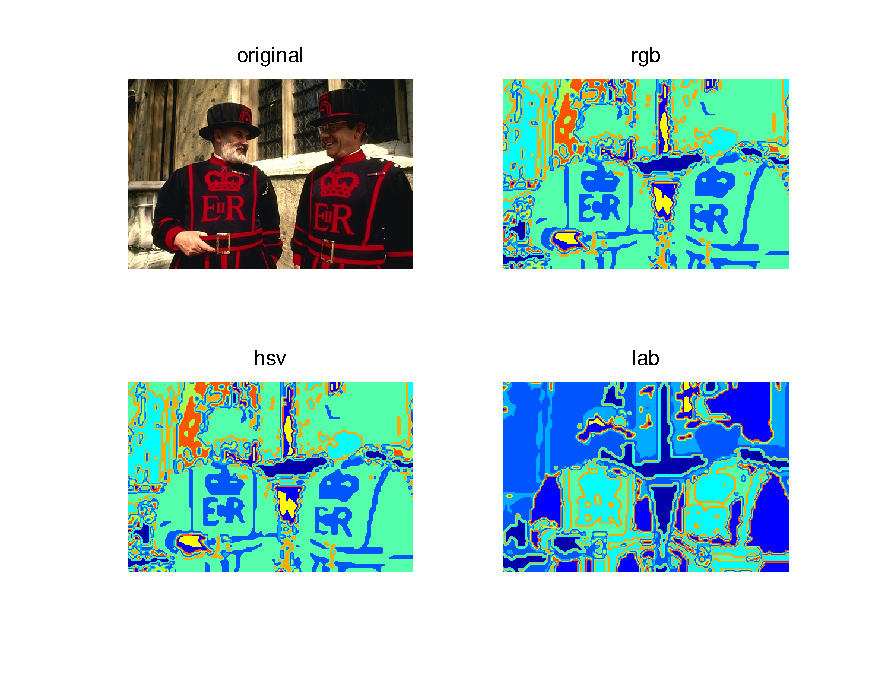
\includegraphics[scale=0.6]{jera.eps}
\end{center}
   \caption{Método jerarquico y espacios de color con h=10. }
\label{fig:long}
\label{fig:onecol}
\end{figure}
%%%%%%%%%%%%%%%%%%%%%%%%%%%%%%%%%%%%%%%%55

\begin{itemize}
 \item Evaluación
\end{itemize}
Se implementó el código boundaryBench de Pablo Arbelaez $<arbelaez@eecs.berkeley.edu>$\cite{5557884}, para evaluar las diferentes técnicas de segmentación propuestas y 
aplicadas a las las imágenes de test de la base de datos de berkeley. Como resultado se tiene la gráfica de precisión y cobertura para poder dar un estimado de qué tan bueno
o malo es el método. Los resultados se encuentran en las figuras 7, 8, 9, 10 y 11.
\begin{figure}[h]
\begin{center}
   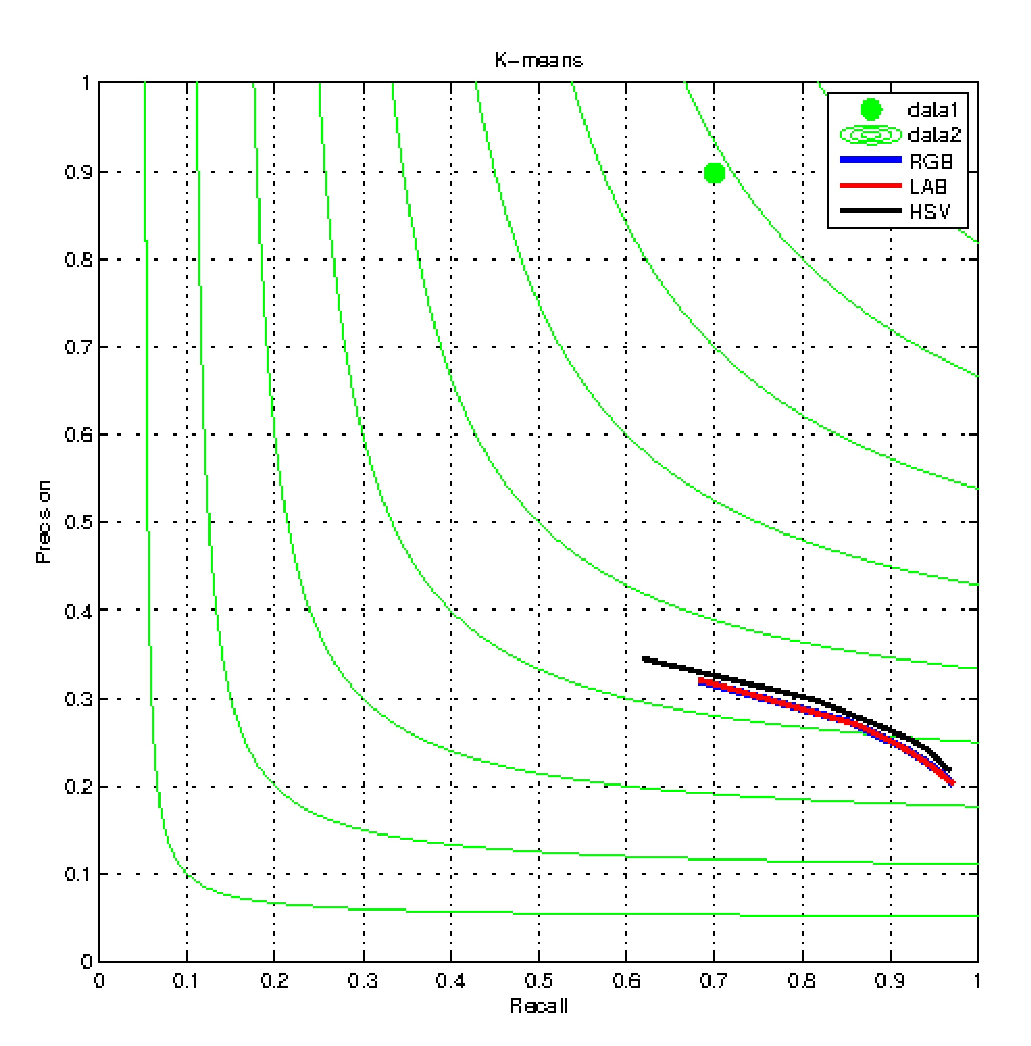
\includegraphics[scale=0.4]{K-meansiso.eps}
\end{center}
   \caption{Evaluación de los espacios de color y k-means con la gráfica de precisión y cobertura.}
\label{fig:long}
\label{fig:onecol}
\end{figure}

\begin{figure}[ht]
\begin{center}
 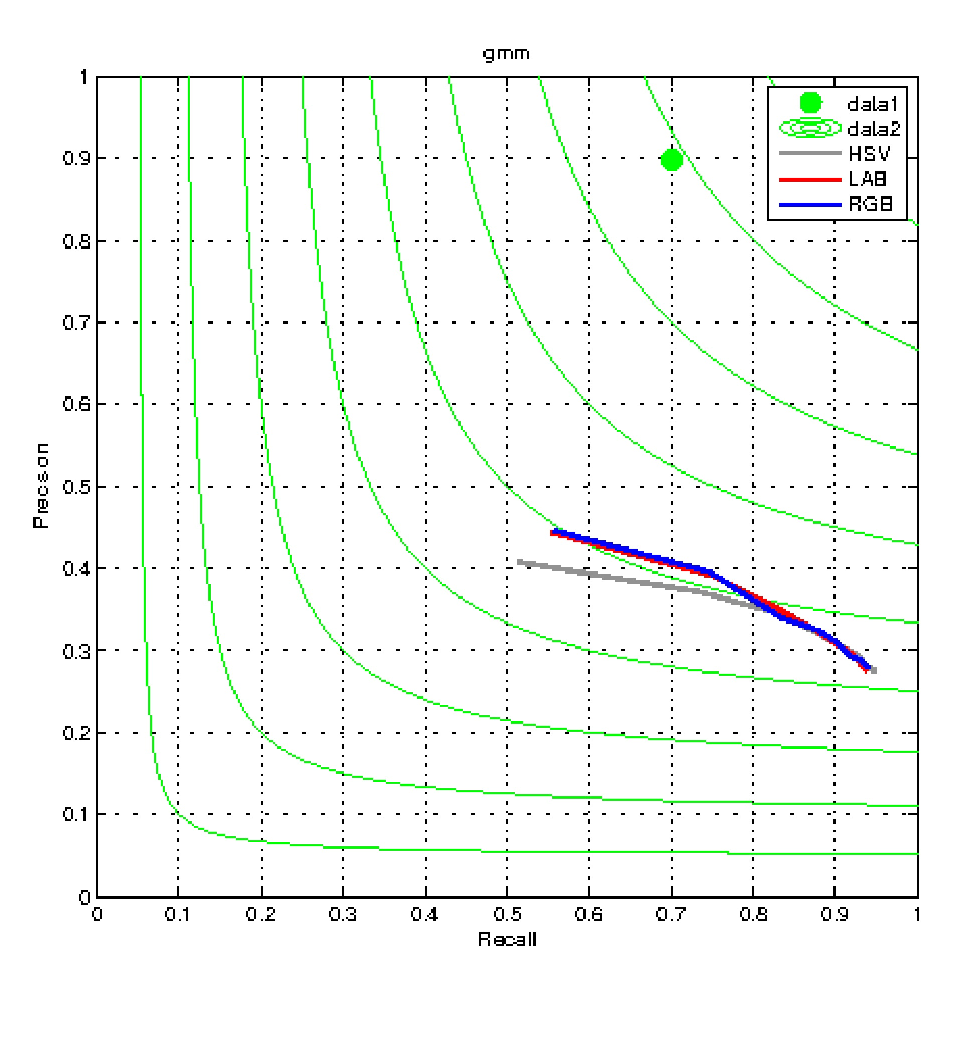
\includegraphics[scale=0.4]{gmmis.eps}
\end{center}
   \caption{Evaluación de los espacios de color y gmm con la gráfica de precisión y cobertura.}
\label{fig:long}
\label{fig:onecol}
\end{figure}

\begin{figure}[ht]
\begin{center}
   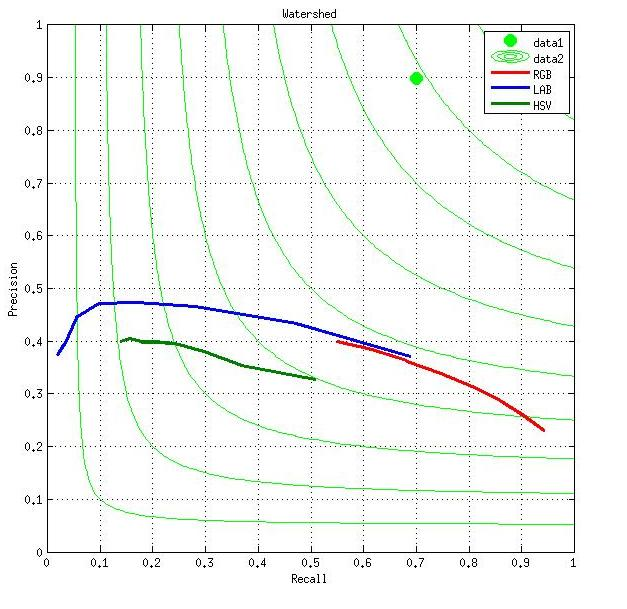
\includegraphics[scale=0.4]{watershed.jpg}
\end{center}
   \caption{Evaluación de los espacios de color y watershed la gráfica de precisión y cobertura. }
\label{fig:long}
\label{fig:onecol}
\end{figure}

\begin{figure}[ht]
\begin{center}
   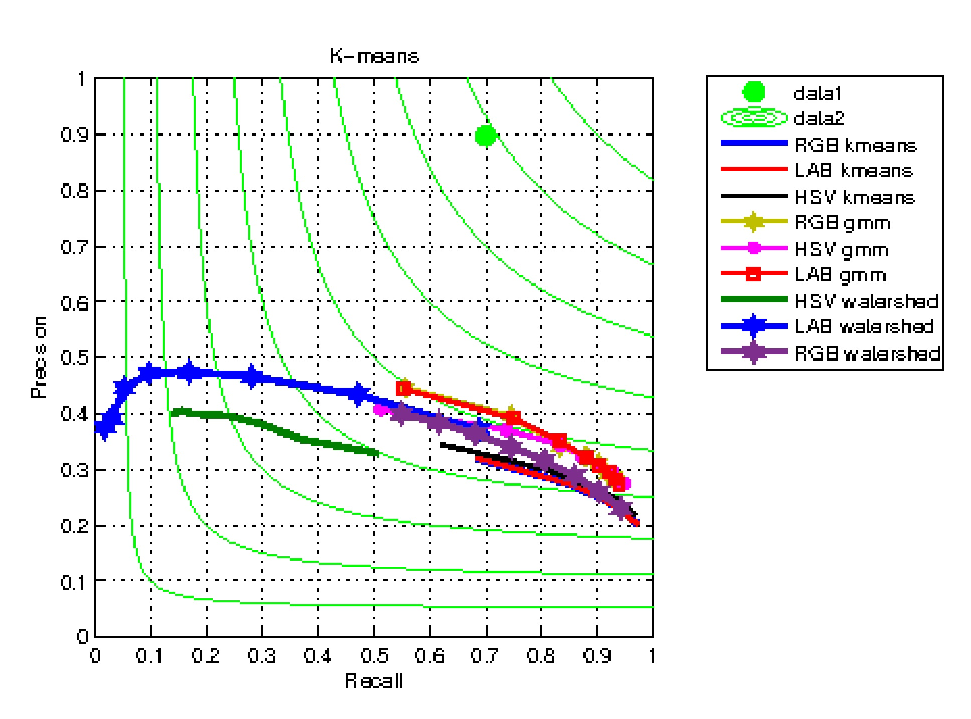
\includegraphics[scale=0.55]{completas.eps}
\end{center}
   \caption{Gráfica comparativa de los resultados de la evaluación para los métodos propuestos. }
\label{fig:long}
\label{fig:onecol}
\end{figure}

\begin{figure}[ht]
\begin{center}
   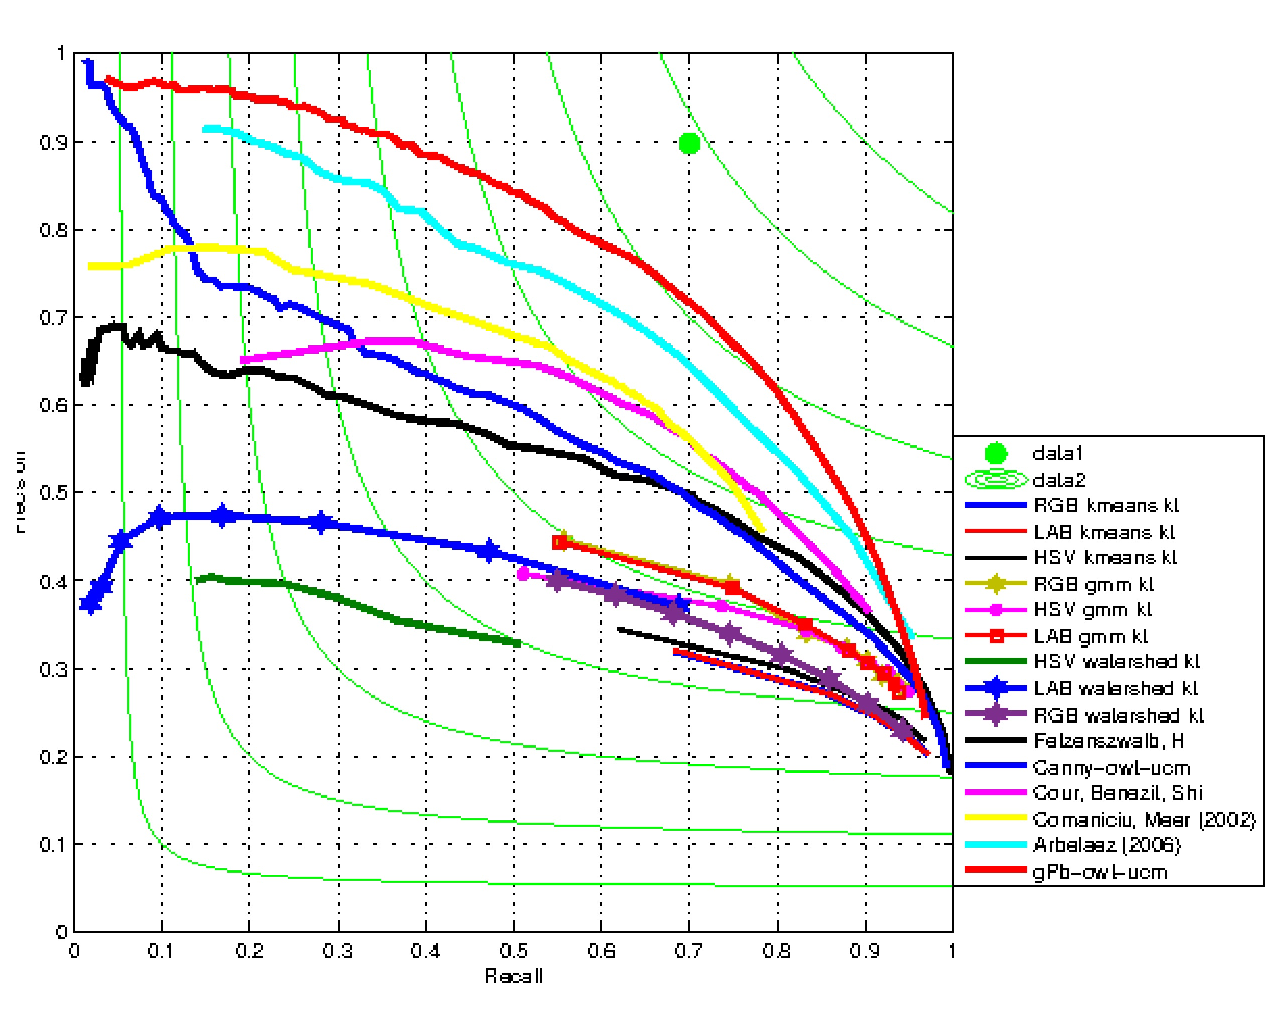
\includegraphics[scale=0.42]{compara1.eps}
\end{center}
   \caption{Resultados de la evaluación de los métodos propuestos vs los métodos propuestos en el mundo. }
\label{fig:long}
\label{fig:onecol}
\end{figure}


\section{Discusión}

Al implementar la función de segmentación para los distintos espacios de representación de color, se observó que los espacios
que involucran la posición espacial no proporcionan una mejor segmentación. Se esperaba que al incluir las posiciones xy
estas dos variables aportaran información a los píxeles de color y así lograr obtener una segmentación sobre el color apoyada en el posicionamiento.
Sin embargo, la segmentación se basó más en el posicionamiento que en los valores de color de la imagen, como se puede observar en la Figura 1 
(parte superior es la segmentación sin tener en cuenta xy y la parte de inferior teniendo encuenta xy),
se pueden comparar los resultados de la segmentación y corroborar lo dicho anteriormente.
\\
\\
Durante la etapa de entrenamiento se observaron los resultados de las segmentaciones para los 4 métodos propuestos y se estimaron los 
rangos adecuados para implementar cada uno de los métodos. Para k-means y gmm se decidió que los valores adecuados están en un rango entre 2 a 16 (ejemplo: Figura 2 y 3 con k=4).
Para el método jerárquico los valores se pueden estimar entre 2 a 30, sin embargo los resultados varían dependiendo de la imagen y no son muy buenos comparados con los de k-means 
y gmm (Figura 5 y 6). Para watershed los rangos se estimaron valores entre 20 a 90, pero a pesar de tener un rango amplio los resultados presentan sobresegmentación y a medida que se aumenta el nivel se pierden segmentos 
importantes como se evidencia en la Figura 4. 
\\
\\
Es difícil decir que espacio de representación de color y qué técnica de segmentación es la mejor con solo el análisis visual.
Por ello es necesario evaluar las distintas técnicas con un método de evaluación; en nuestro se usó caso boundari bench para obtener la gráfica de 
precisión-cobertura.
\\
\\
Para la evaluación de los resultados se analizó cada método de manera individual para estimar cuál espacio de color es el más oportuno para utilizar en la segmentación
y como se puede observar en la Figura 7, para k-means los resultados de lab y rgb son muy parecidos y los resultados de hsv son un poco mejores, dado que maneja una precisión
mayor que la de lab y rgb, y además presenta un rango mayor de cobertura aunque al final la cobertura es mayor para lab.
En el caso de gmm (Figura 8) el espacio hsv presenta peor rendimiento y rgb-lab siguen presentando características similares en la respuesta.
Finalmente se evaluó watershed (Figura 9) encontrando un amplio rango de cobertura con lab y mayor precisión pero en ese instante la cobertura es mínima, en rgb se encontró la mayor cobertura de gmm.
\\
\\
En la Figura 10 se muestran los resultados simultáneos de la función propuesta y se observa que la gráfica roja que representa gmm-lab es aparentemente el mejor resultado, y la manera de comprobar esto es mediante la Tabla 1,
que nos muestra medias estadísticas de las gráficas consideradas como los mejores resultados para cada método. De esa manera es posible evidenciar que gmm-lab tiene el mayor ODS e IDS entendido como la escala optima para el conjunto de datos y la escala optima de imágen.
Sin embargo al comparar los resultados obtenidos con los métodos propuestos con los mejores métodos desarrollados en el mundo\cite{5557884}, se evidencia que la metodología propuesta se queda corta con lo que va hasta el momento en el mundo, como es el caso de gPb-owl-ucm con una alta cobertura y precisión.  


\begin{table}
\begin{center}
\begin{tabular}{|l|l|l|l|l|}
\hline
Method & ODS & OIS & Área & th \\
\hline\hline
Watershed-lab & 0.48 & 0.51 & 0.29 & 1.1 \\
Gmm-lab & 0.52 & 0.58 & 0.15 & 2.0 \\
Kmeans-hsv & 0.44 & 0.49 & 0.1 & 1.30\\
gPb-owt-ucm & 0.73 & 0.76 & 0.73 &   - \\
\hline
\end{tabular}
\end{center}
\caption{Resultados de la mejor gráfica por método}
\end{table}

\section{Conclusiones}

De los métodos mencionados anteriormente se puede inferir al visualizar los resultados de la segmentación que técnicas como watershed al 
manejar un mayor rango en los datos es posible tener una mayor precisión en algunos casos, en contraste con los métodos donde se toman pocos
valores de agrupamiento y no muy diferenciables entre ellos.  
\\
\\
Los resultados de segmentación incluyendo coordenadas no mejoran la clasificaión de objetos.
Por el contrario se enfocan más en la segmentación de cuadrantes.\
\\
\\
A pesar de que gmm fue el método que tomó más tiempo que las demás técnicas en segmentar imágenes, los resultados fueron mejores en el espacio de color lab, por tanto,
para proyectos básicos de segmentación se puede utilizar facilmente un método como gmm-lab simple de implementar.
%-----------------------------------------------------------------------
%%----
{\small
\bibliographystyle{apalike}
\bibliography{ref1.bib}



\end{document}
